\section{Experiments in the dolphin data}
This study investigated maximal alpha-cliques within a dolphin social network data using an alpha threshold of 0.8, with cliques comprising at least five dolphins. The analysis identified four maximal cliques, each reflecting unique gender distributions, providing insights into potential social dynamics influenced by gender within the dolphin community.

\subsection{Maximal Alpha-Clique 1}
\textbf{Composition}: Jonah, MN105, MN83, Patchback, Topless, and Trigger. \\
\textbf{Gender Distribution}: This clique predominantly consists of males, with five males and one female. \\
\textbf{Interpretation}: The male dominance within this group suggests that male dolphins in this network may form strong social bonds with limited female presence. Such a configuration could indicate either a preference for male companionship or shared behaviors and social interactions unique to male dolphins within this subset of the network.
\begin{figure}[H]
    \centering
    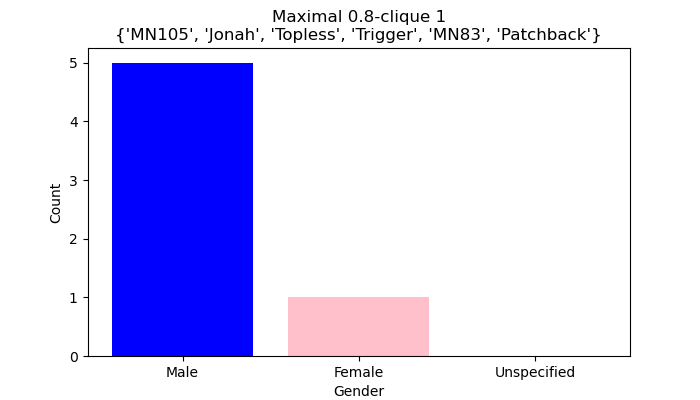
\includegraphics[width=1.0\textwidth]{clique_1.png}
    \caption{Clique 1}
    \label{fig:clique_1}
\end{figure}

\subsection{Maximal Alpha-Clique 2}
\textbf{Composition}: Grin, Hook, SN4, SN63, Scabs, and Stripes. \\
\textbf{Gender Distribution}: All members in this clique are female. \\
\textbf{Interpretation}: The exclusivity of female members in this clique suggests a gender-based social structure, where female dolphins are inclined to form tightly-knit groups. This homogeneous grouping may reflect social bonding patterns or cooperative behaviors specific to females, potentially serving as mechanisms for support or protection within the dolphin community.
\begin{figure}[H]
    \centering
    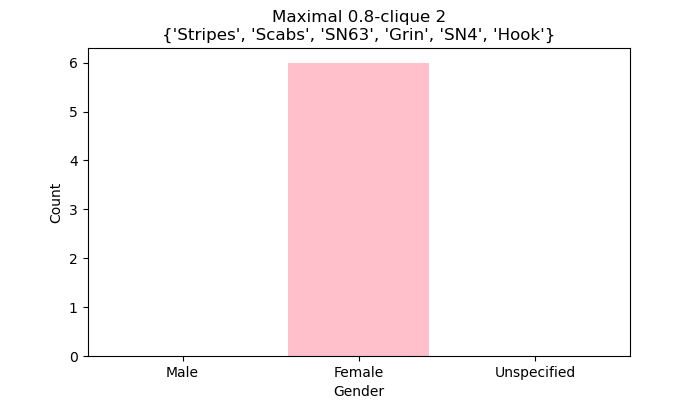
\includegraphics[width=1.0\textwidth]{clique_2.png}
    \caption{Clique 2}
    \label{fig:clique_2}
\end{figure}

\subsection{Maximal Alpha-Clique 3}
\textbf{Composition}: DN21, Feather, Gallatin, SN90, Upbang, and Web. \\
\textbf{Gender Distribution}: This clique is exclusively male. \\
\textbf{Interpretation}: The existence of a male-only clique, similar to Clique 1 but with a complete absence of females, highlights a pattern of strong male alliances. The homogeneous nature of this clique may suggest a stable network of male friendships or alliances that play a role in male social strategies, possibly for cooperation in social or territorial behaviors within their community.
\begin{figure}[H]
    \centering
    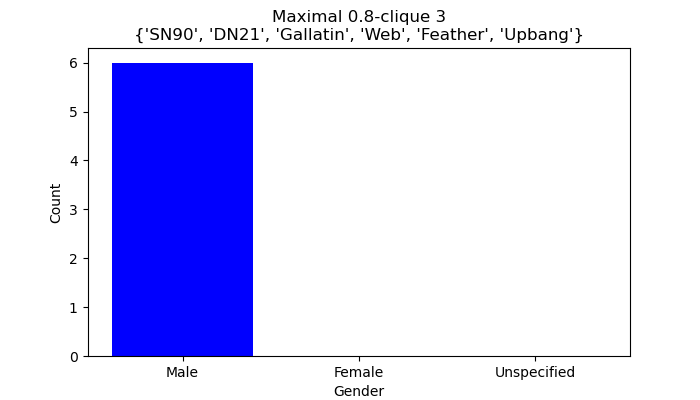
\includegraphics[width=1.0\textwidth]{clique_3.png}
    \caption{Clique 3}
    \label{fig:clique_3}
\end{figure}

\subsection{Maximal Alpha-Clique 4}
\textbf{Composition}: DN21, Feather, Gallatin, Jet, and Web. \\
\textbf{Gender Distribution}: Like Clique 3, this group is exclusively male. \\
\textbf{Interpretation}: This smaller, all-male clique demonstrates a tightly interconnected subgroup, as indicated by its higher internal connectivity (fs = 1.00). This high level of connectivity suggests an exceptionally stable social structure within the male subgroup, reinforcing the hypothesis that male dolphins form strong, exclusive bonds that could serve social or survival functions within the community.
\begin{figure}[H]
    \centering
    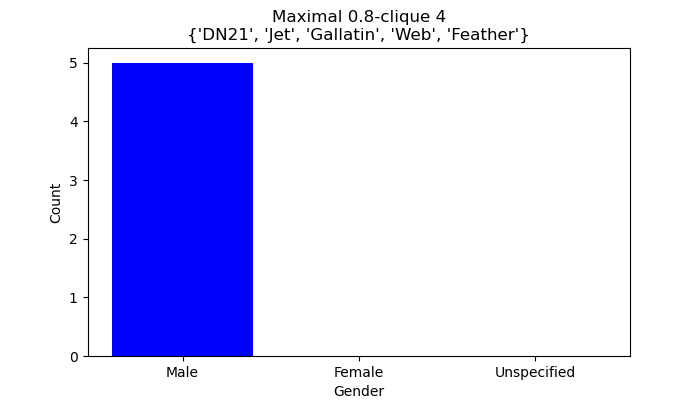
\includegraphics[width=1.0\textwidth]{clique_4.png}
    \caption{Clique 4}
    \label{fig:clique_4}
\end{figure}

The observed gender distributions within the maximal alpha-cliques reveal notable patterns of gender-based social structuring in the dolphin community. Specifically, cliques tend to exhibit gender homogeneity, with all-female or all-male groups forming more frequently than mixed-gender groups. This tendency suggests that gender plays a significant role in the formation and cohesion of social subgroups within the dolphin network, potentially influenced by behaviors, social preferences, or survival strategies specific to each gender.

In conclusion, this analysis underscores the complexity of dolphin social behavior, emphasizing the influence of gender on subgroup formation within their networks. Based on the assumption that the graph is naturally connected, it would be interesting to run the analysis on a more accurate weighted graph to see the difference between an unweighted and a weighted graph. Intuitively, the weighted graph would produce a more accurate clustering. Additionally, a comparison to the clustering of other sea mammals would produce better interpretation of the result.